% IEEE Conference Template for System/Engineering Papers (Codebase-grounded)
\documentclass[conference]{IEEEtran}

\IEEEoverridecommandlockouts

%%%%%%%%%%%%%%%%%%%%%%%%%%%%%%%%%%%%%%%%%
% PACKAGES
%%%%%%%%%%%%%%%%%%%%%%%%%%%%%%%%%%%%%%%%%
\usepackage{cite}
\usepackage{enumitem}
\usepackage{amsmath,amssymb,amsfonts}
\usepackage{algorithm}
\usepackage{algorithmic}
\usepackage{graphicx}
\usepackage{textcomp}
\usepackage{xcolor}
\usepackage{forest}
\usepackage{tikz}
\usepackage{adjustbox}
\usepackage{url}
\usepackage{pgfplots}
\usepackage{booktabs}
\usepackage{colortbl}
\usetikzlibrary{shapes.geometric,arrows,positioning,fit,backgrounds,calc,decorations.pathreplacing,decorations.markings,patterns,matrix,chains}
\usepackage{threeparttable}
\usepackage{cuted}

\makeatletter
\newcommand{\linebreakand}{%
  \end{@IEEEauthorhalign}
  \hfill\mbox{}\par
  \mbox{}\hfill\begin{@IEEEauthorhalign}
}
\makeatother

\definecolor{qubitblue}{RGB}{70,130,180}
\definecolor{controlred}{RGB}{220,20,60}
\definecolor{aigreen}{RGB}{50,150,50}
\definecolor{quantumpurple}{RGB}{128,0,128}
\definecolor{errororange}{RGB}{255,140,0}

%%%%%%%%%%%%%%%%%%%%%%%%%%%%%%%%%%%%%%%%%
% DOCUMENT BEGINS
%%%%%%%%%%%%%%%%%%%%%%%%%%%%%%%%%%%%%%%%%
\begin{document}

\title{[Your Paper Title: Project/System Name + Specific Focus]}

\author{
    \IEEEauthorblockN{
        [Author 1]\textsuperscript{*, a},
        [Author 2]\textsuperscript{a}
    }
    \IEEEauthorblockA{
        \textsuperscript{a}[Institution, Country]
    }
    \IEEEauthorblockA{
        *Corresponding Email: [email@example.com]
    }
}

\maketitle

\begin{IEEEkeywords}
[Keyword 1], [Keyword 2], [Keyword 3], [Keyword 4]
\end{IEEEkeywords}

\begin{abstract}
[Single paragraph (150--250 words): problem, system, key contributions, evidence-backed results (if measured), and main takeaways. Avoid citations in the abstract.]
\end{abstract}

\section{Introduction}
[Context and problem statement. Explicitly list contributions as evidence-backed claims. Cite frameworks or prior systems when needed.]

\section{System Overview}
[High-level architecture and data/control flow. Include a diagram that matches the actual implementation.]

\begin{figure}[t]
    \centering
    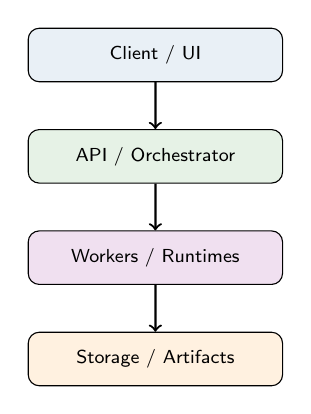
\begin{tikzpicture}[
        scale=0.85, transform shape,
        node distance=0.7cm,
        box/.style={rectangle, rounded corners, draw, fill=#1!12, text=black,
            minimum width=3.8cm,
            minimum height=0.8cm,
            align=center, font=\sffamily\footnotesize}
    ]
        \node[box=qubitblue] (client) {Client / UI};
        \node[box=aigreen, below=of client] (api) {API / Orchestrator};
        \node[box=quantumpurple, below=of api] (workers) {Workers / Runtimes};
        \node[box=errororange, below=of workers] (storage) {Storage / Artifacts};

        \draw[->, thick] (client) -- (api);
        \draw[->, thick] (api) -- (workers);
        \draw[->, thick] (workers) -- (storage);
    \end{tikzpicture}
    \caption{[Architecture overview diagram. Replace nodes with real components from the codebase.]}
    \label{fig:arch}
\end{figure}

\section{Architecture and Components}
[Map components to real modules and responsibilities.]

\subsection{Component Map}
[Provide a table mapping component $\rightarrow$ module path(s) / package(s).]

\subsection{Backend / Core Services}
[Describe core services, APIs, data models, and execution model.]

\subsection{Frontend / UX (if applicable)}
[Describe UI architecture, state management, and key user workflows.]

\subsection{Infrastructure / Execution (if applicable)}
[Describe queues/workers, scheduling, caching, and deployment assumptions.]

\section{End-to-End Workflow}
[Describe the primary workflows with concrete steps grounded in the call graph or docs. Include failure and retry paths.]

\section{Reliability, Safety, and Observability}
[Evidence-backed mechanisms only: retries, idempotency, audit logs, privacy, policy checks, metrics, alerts.]

\section{Evaluation}
[Report measured results if available; otherwise present an explicit evaluation plan and missing artifacts.]

\section{Related Work}
[Position against closest systems and cite key frameworks. All citations must be verified.]

\section{Limitations and Future Work}
[Call out limitations honestly; propose concrete next steps without overstating.]

\section{Conclusion}
[Summarize contributions and takeaways; do not introduce new claims without evidence.]

\bibliographystyle{ieeetr}
\bibliography{ref}

\end{document}

